\documentclass[10.5pt
%,draft
]{article}


\usepackage{ctex}
\usepackage{graphicx}
\usepackage{amsmath}
\usepackage{xcolor}
\usepackage{physics}
\usepackage{hyperref}
\hypersetup{
    colorlinks=true,
    linkcolor=Blue4Link,
    filecolor=magenta,      
    urlcolor=cyan,
    pdfauthor=徐均益
    }
\definecolor{Blue4Link}{RGB}{46,49,146}
\definecolor{myOrange}{RGB}{178,76,0}
\definecolor{green4eye}{RGB}{0,120,2}%
\definecolor{blue4eye}{RGB}{1,126,218}%
\definecolor{cyan4eye}{RGB}{31,186,190}%
\definecolor{myhighlight}{RGB}{255,214,161}
\definecolor{mybackground}{RGB}{204,232,207}
\usepackage{geometry}
\usepackage{natbib}
\usepackage{subcaption}

\renewcommand{\refname}{参考文献}
\renewcommand{\figurename}{图}
\renewcommand{\abstractname}{摘要}

\def\due{2023 年 4 月 26 日周一 8:40}
\def\Term{2023 年春季}
\def\Course{磁流体力学的数值模拟方法}

\title{一维气体激波管问题 --- 第 3 次作业\footnote{\Term\Course}}

\author{徐均益\footnote{ID: SA22214015 Email: jyxu@mail.ustc.edu.cn}
  \and
  余航\footnote{ID: SA22168021 Email: yh131996@mail.ustc.edu.cn}
  \and
  陈宇韬\footnote{ID: SA22214014 Email: chenyut@mail.ustc.edu.cn}
}

\date{%
\scriptsize%
%CAS Key Laboratory for Basic Plasma Physics, School of Earth and Space Sciences,
%\\
%University of Science and Technology of China, Hefei, Anhui 230026, China
中国科学技术大学核科学技术学院, 合肥 230026 \\
中国科学技术大学物质科学研究院等离子所, 合肥 230026
%
}

\begin{document}

\maketitle

\begin{abstract}
课程《磁流体力学的数值模拟方法》的第三次作业,讨论一维气体激波管问题的有限差分数值解法,分别使用守恒型方程的\textit{LaxWendroff}格式,非守恒型的\textit{Upwind}格式和\textit{Minmod}格式,通过理论分析和实验编程,讨论该方程的物理解和数值解的特性,并分析流体中不同波模的物理和数值特性。 

\end{abstract}

\section{引言}
一维气体激波管问题是计算流体力学中的经典问题,也是为数不多的存在精确解的问题,
常以此算例检测数值格式,
% 常用来检测算例来检验数值格式,
% 这使得学习研究和在此类问题上实现各种数值方法具有现实意义。
方便我们进一步学习研究各种数值方法,
同时一维气体激波管所使用的物理方程为连续性方程、动量方程、能量方程,
% 可以写成三个守恒形式的方程,也意味着取合适的迭代矩阵,能使其数学描述为双曲守恒形式。
可以写成守恒形式,
% 也意味着选择合适的迭代矩阵,能使其数学描述为双曲守恒形式。
也意味着选择合适的迭代矩阵,能够化为双曲守恒形式。
可以检验各种方法在守恒形式和非守恒形式下的异同。
本次作业只考虑无粘滞的理想气体状态方程下的一维激波问题。

\section{理论基础介绍}
\subsection{守恒形式}
\subsubsection{方程介绍}
考察一维多方气体 Euler 方程
\begin{equation}
\frac{\partial w}{\partial t} + \frac{\partial f(w)}{\partial
x}= 0\label{Eqn:Euler},
\end{equation}
的 Riemann 问题 (一维气体激波管问题),其中
\begin{align}
w =& \left[\begin{array}{c}
\rho\\
m\\
E
\end{array}\right],
\\
f(w) =& u w + \left[\begin{array}{c}
0\\
p\\
p u
\end{array}\right] = \left[\begin{array}{c}
m
\\
(\gamma - 1) E + \frac{3 - \gamma}{2} \frac{m^2}{\rho}
\\
(\gamma E - \frac{\gamma - 1}{2} \frac{m^2}{\rho}) \frac{m}{\rho}
\end{array}\right],
\\
m =& \rho u,
\\
p =& (\gamma - 1)(E - \frac{1}{2} \rho u^2).
\end{align}
这里, $\rho$, $m$ 和 $E$ 分别是密度, 质量流和能量. 
其对应的三个方程分别为质量守恒方程,动量守恒方程和能量守恒方程。
守恒形式可以采用\textit{LaxWendroff}格式设计实验。

\subsubsection{特征向量计算}\label{Appendix}
将方程~\eqref{Eqn:Euler} 可以写成如下形式
\begin{align}
\frac{\partial w}{\partial t} + \vb*A \vdot \frac{\partial w}{\partial
x}= 0,\label{Eqn:Euler2}
\end{align}
守恒形式下 $\vb*A$ 的表达式
\begin{align*}
\vb*A =& \frac{\partial f}{\partial w} = \left[\begin{array}{ccc} 0 & 1 & 0
\\
\frac{1}{2} (\gamma  - 3) u^2 & -(\gamma - 3) u & \gamma - 1
\\
(\gamma - 1) u^3 - \gamma \frac{u}{\rho} E & \gamma \frac{1}{\rho} E-\frac{3}{2} (\gamma
- 1) u^2 & \gamma u
\end{array}
\right]
\end{align*}
左右特征向量
\begin{align*}
\vb*R =& \left[\begin{array}{ccc} 1 & 1 & 1
\\
u - c & u & u + c
\\
H - u c & \frac{1}{2} u^2 & H + u c
\end{array}
\right]
\\
\vb*L =& \frac{\gamma - 1}{2 c^2} \left[\begin{array}{ccc} \frac{1}{2} u \left(u + \frac{2
c}{\gamma - 1}\right) & -\left(u + \frac{c}{\gamma - 1}\right) & 1
\\
2(H - u^2) & 2 u & - 2
\\
\frac{1}{2} u \left(u - \frac{2 c}{\gamma - 1}\right) & -\left(u - \frac{c}{\gamma -
1}\right) & 1
\end{array}
\right]
\end{align*}
其中
\begin{align*}
H =& \frac{E + p}{\rho} = \frac{c^2}{\gamma - 1} + \frac{1}{2} u^2,
\\
c^2 =& \gamma \frac{p}{\rho}.
\end{align*}

\subsection{非守恒形式}
式~\eqref{Eqn:Euler} 的非守恒形式为
\begin{align}
\pdv{\vb u}{t} + \vb*B \vdot \pdv{\vb u}{x} = 0,
\label{Eqn:Euler3}
\end{align}
其中
\begin{align}
\vb u = [u_j] = \left[\begin{array}{c}\rho\\ u\\ p\end{array}\right], \quad \vb*B = [B_{ij}] = \left[\begin{array}{ccc}u & \rho & 0\\
0 & u & 1/\rho\\ 0 & \gamma p & u\end{array}\right]
\end{align}
此时方程~\eqref{Eqn:Euler2} 与方程~\eqref{Eqn:Euler3} 虽然形式看起来相同,
同时代入后得到的三个方程也相同,
但是因为方程~\eqref{Eqn:Euler2} 形式上可以化成守恒形式~\eqref{Eqn:Euler},
而方程~\eqref{Eqn:Euler3} 无法化成守恒形式。因此两个方程虽然表示的是同一个物理现象但是一个为守恒形式一个为非守恒形式,分别适用于不同的差分格式。

其中,矩阵 $\vb*B$ 的特征值为 $u-a$, $u$, $u+a$ ($a^2 = \gamma p/\rho$), 对应的左右特征向量矩阵为 $\vb*L$ 和 $\vb*R$ 写为
\begin{align}
\vb*L =& [L_{ij}] = \left[\begin{array}{ccc}0 & -\rho a & 1\\ a^2 & 0 & -1\\ 0 & \rho a & 1\end{array}\right],
\\
\vb*R =& [R_{ij}] = \left[\begin{array}{ccc}\frac{1}{2a^2} & \frac{1}{a^2} & \frac{1}{2a^2}\\
-\frac{1}{2\rho a} & 0 & \frac{1}{2\rho a}\\ \frac{1}{2} & 0 & \frac{1}{2}\end{array}\right]
\end{align}
波模分解的方程为
\begin{align}
\sum_j \left\{L_{ij} \frac{\partial u_j}{\partial t} + \lambda_i L_{ij} \frac{\partial u_j}{\partial
x}\right\} = 0,
\end{align}
其中
\begin{align}
\lambda_i =
\left[\begin{array}{c}u-a \\ u\\ u+a\end{array}\right]
\end{align}
在变换回原变量方程的形式, 即
\begin{align}
\sum_i \sum_j \left\{R_{ki} L_{ij} \frac{\partial u_j}{\partial t} + R_{ki} \lambda_i L_{ij}
\frac{\partial u_j}{\partial x}\right\} = 0,
\end{align}
并利用 $\sum_i R_{ki} L_{ij} = \delta_{kj}$, 我们有
\begin{align}
\frac{\partial u_k}{\partial t} + \sum_i \sum_j \left\{R_{ki} \lambda_i L_{ij} \frac{\partial
u_j}{\partial x}\right\} = 0,
\end{align}
迎风格式为
\begin{align}
u_{k,l}^{n+1} =& u_{k,l}^n \nonumber\\
& - \frac{\Delta t}{\Delta x} \sum_i \sum_j \left\{\text{sgn}(\lambda_{i,l}^n)
 \lambda_{i,l}^n R_{ki,l}^n L_{ij,l}^n \left[u_{j,l}^n - u_{j,l-\text{sgn}(\lambda_{i,l}^n)}^n\right]\right\}
\end{align}
其中下角标 $l$ 对应于空间格点位置, 其他下角标对应于分量.

对于非守恒方程可以用迎风格式和\textit{minmod}格式。

\section{实验与结果分析}
\subsection{初始值设计}
对方程
\begin{align}
\frac{\partial \vb w}{\partial t} + \frac{\partial \vb F}{\partial x} = 0
\end{align}
在$t = 0$时刻有
\begin{align}
w(x,t)|_{t=0} = \left\{ \begin{array}{ll}
W_L, & \quad x < 0 \\
W_R, & \quad x > 0
\end{array} \right.
\end{align}
为和经典数值计算结果比较,取文献 \citet{Harten1983} 中的值, 即 $\gamma=1.4$, 和
\begin{align}
    W_L = \left[\begin{array}{l}
    0.445\\
    0.311\\
    8.928
    \end{array}\right], \quad W_R = \left[\begin{array}{l}
    0.5\\
    0\\
    1.4275
    \end{array}\right]
\end{align}
\subsection{精确解格式}
精确解由附件Hydrodynamics.xlsx中提供,其最终形式为分为五段的分段函数,具体形式如下
\begin{align}
\rho = \left\{ \begin{array}{ll}
0.445, & \quad x < v_1 t \\
\qty(x-v_1 t)\dfrac{0.345 - 0.445}{v_2 t - v_1 t} + 0.445, & \quad v_1 t < x < v_2 t \\
0.345, & \quad v_2 t< x < v_3 t \\
1.304, & \quad v_3 t< x < v_4 t \\
0.500, & \quad x > v_4 t
\end{array} \right.
\end{align}
\begin{align}
m = \left\{ \begin{array}{ll}
0.311, & \quad x < v_1 t \\
\qty(x-v_1 t)\dfrac{0.527 - 0.311}{v_2 t - v_1 t} + 0.311, & \quad v_1 t < x < v_2 t \\
0.527, & \quad v_2 t< x < v_3 t \\
1.994, & \quad v_3 t< x < v_4 t \\
0.000, & \quad x > v_4 t
\end{array} \right.
\end{align}
\begin{align}
E = \left\{ \begin{array}{ll}
8.928, & \quad x < v_1 t \\
\qty(x-v_1 t)\dfrac{6.570 - 8.928}{v_2 t - v_1 t} + 8.928, & \quad v_1 t < x < v_2 t \\
6.570, & \quad v_2 t< x < v_3 t \\
7.691, & \quad v_3 t< x < v_4 t \\
1.428, & \quad x > v_4 t
\end{array} \right.
\end{align}
其中$v_1 = -2.633$, $v_2 = -1.636$, $v_3 = 1.529$, $v_4 = 2.480$
\subsection{\textit{Lax-Wendroff}格式}
\textit{Lax-Wendroff}格式适用于守恒型方程
\begin{align}
\frac{\partial \vb w}{\partial t} + \frac{\partial \vb F}{\partial x} = 0
\end{align}
其中差分格式为
\begin{align}
u_j^{n+1} =& u_j^n - \frac{\Delta t}{2\Delta x} (F_{j+1}^n - F_{j-1}^n) \nonumber\\
& + \frac{\Delta t^2}{2\Delta x^2} \left[A_{j+1/2}^n (F_{j+1}^n-F_j^n) - A_{j-1/2}^n (F_j^n -
F_{j-1}^n)\right]
\end{align}
其中 $A = \frac{\partial F}{\partial u}$, $A$ 的表达式见第~\ref{Appendix}~节. 单元边界上的值可以取
\begin{align}
A_{j \pm 1/2}^n = A(u_{j \pm 1/2}^n), \qquad u_{j \pm 1/2}^n = \frac{1}{2} (u_j^n + u_{j \pm 1}^n)
\end{align}
\begin{figure}
\begin{center}
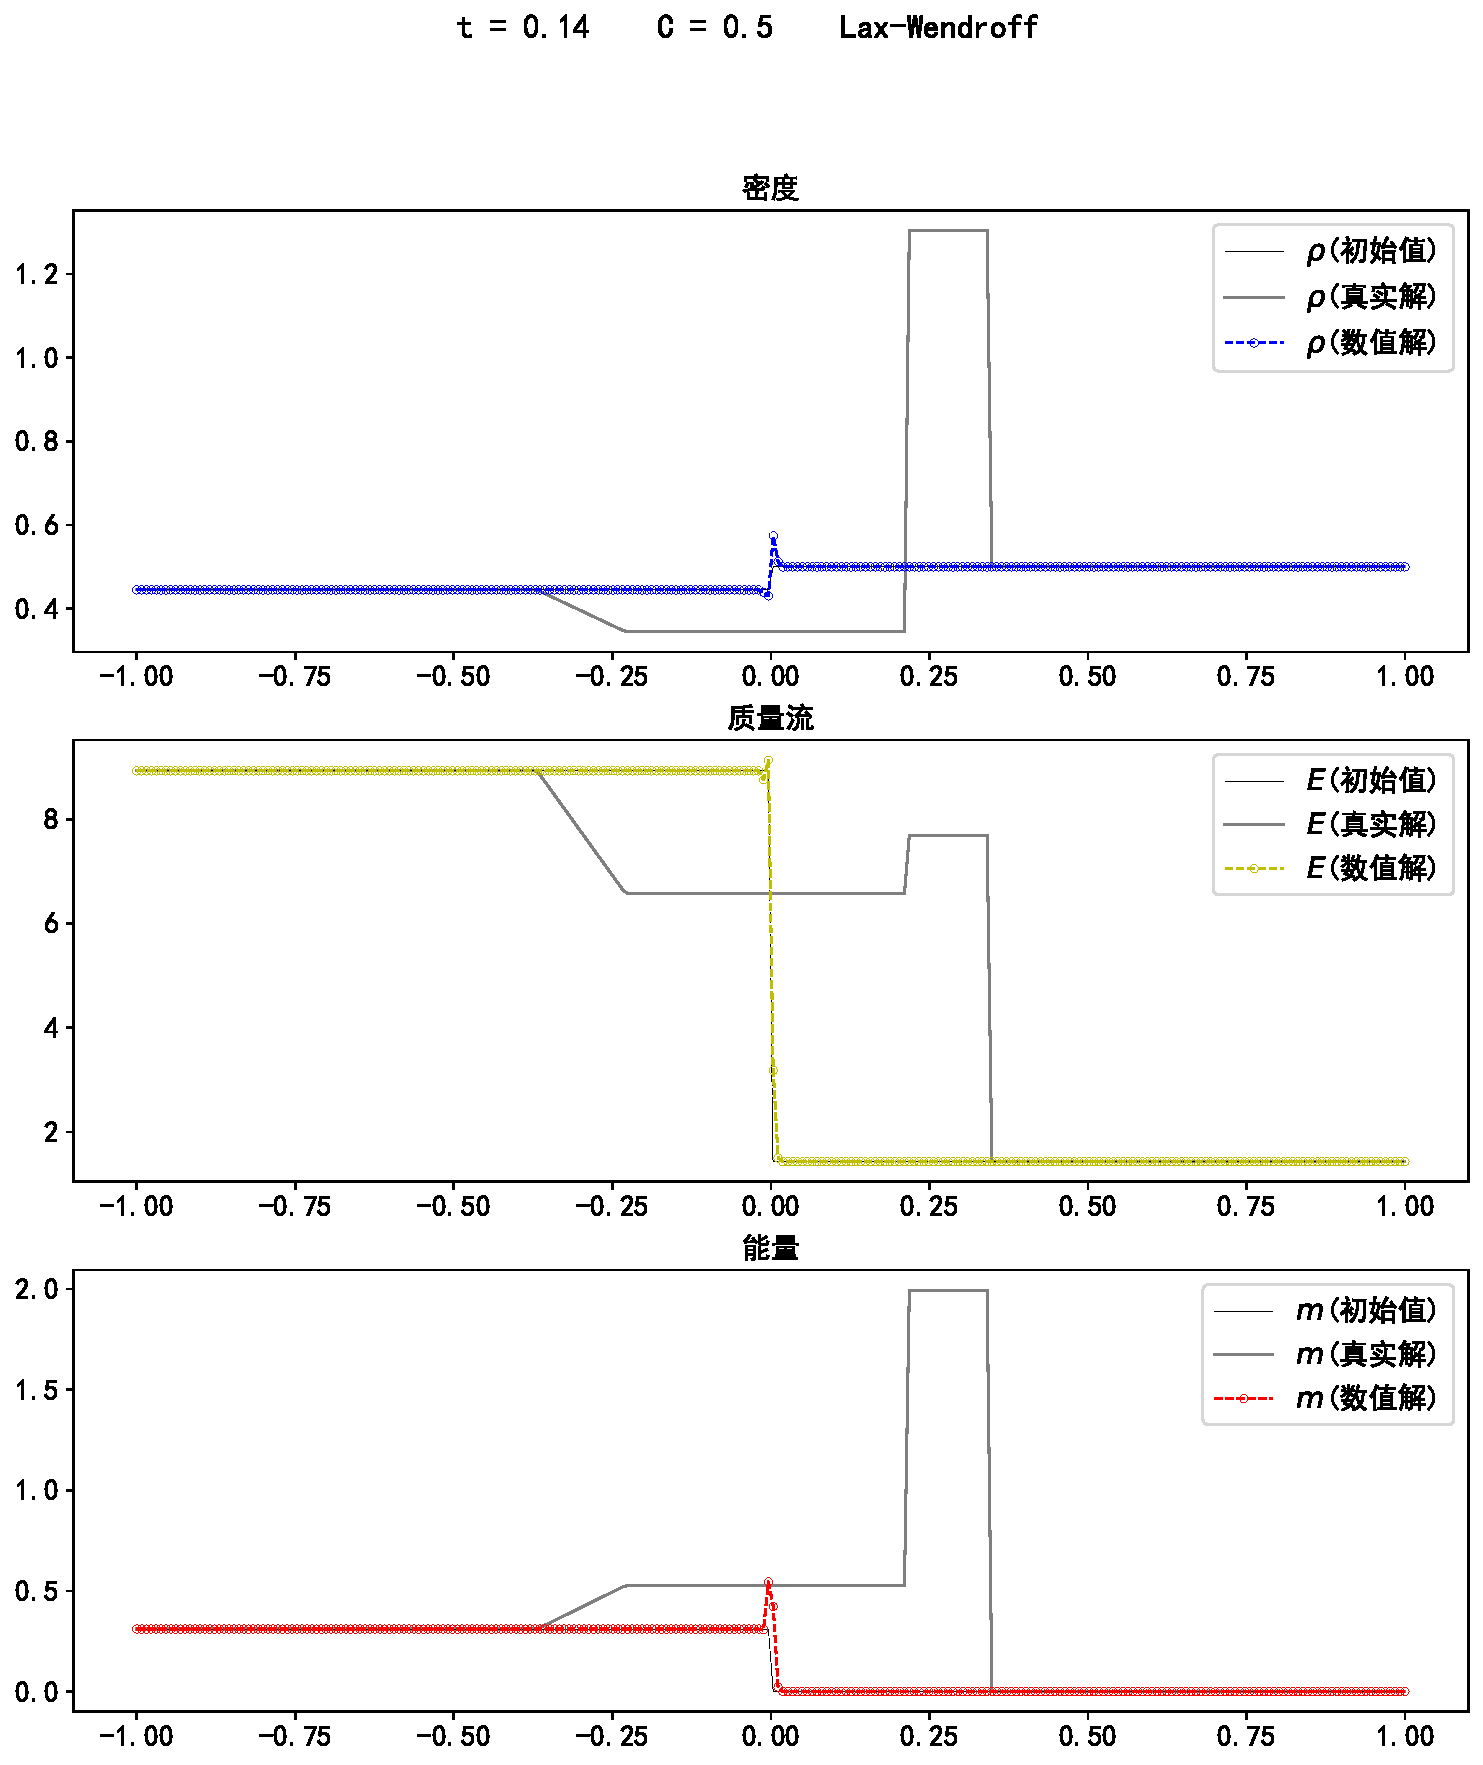
\includegraphics[width=.85\textwidth]{figures/lax_wendroff261.pdf}
\caption{Lax-Wendroff 格式计算结果, 网格点数为 261. \textbf{从上到下分别是密度 $\rho$, 能量 $E$ 和质量流 $m = \rho u$.}
其中点线是初值, 虚线 (上面的数据点用符号 $\circ$ 标注) 是 $t=0.14$ 时的数值结果, 实线是对应的真实解.}\label{fig:lax_wendroff}
\end{center}
\end{figure}
\subsection{\textit{Upwind}格式}
\textit{Upwind}格式既适用于守恒型方程,也适用于非守恒方程,本实验设计使用非守恒方程
\begin{align}
\pdv{\vb u}{t} + \vb*B \vdot \pdv{\vb u}{x} = 0
\end{align}
差分形式为
\begin{align}
u_{k,l}^{n+1} =& u_{k,l}^n \nonumber\\
& - \frac{\Delta t}{\Delta x} \sum_i \sum_j \left\{\text{sgn}(\lambda_{i,l}^n)
 \lambda_{i,l}^n R_{ki,l}^n L_{ij,l}^n \left[u_{j,l}^n - u_{j,l-\text{sgn}(\lambda_{i,l}^n)}^n\right]\right\}
\end{align}
因为分解特征值之后,其特征值的物理意义为传播的波速,所以其正负号决定了迎风格式的差分方向。

\begin{figure}
\begin{center}
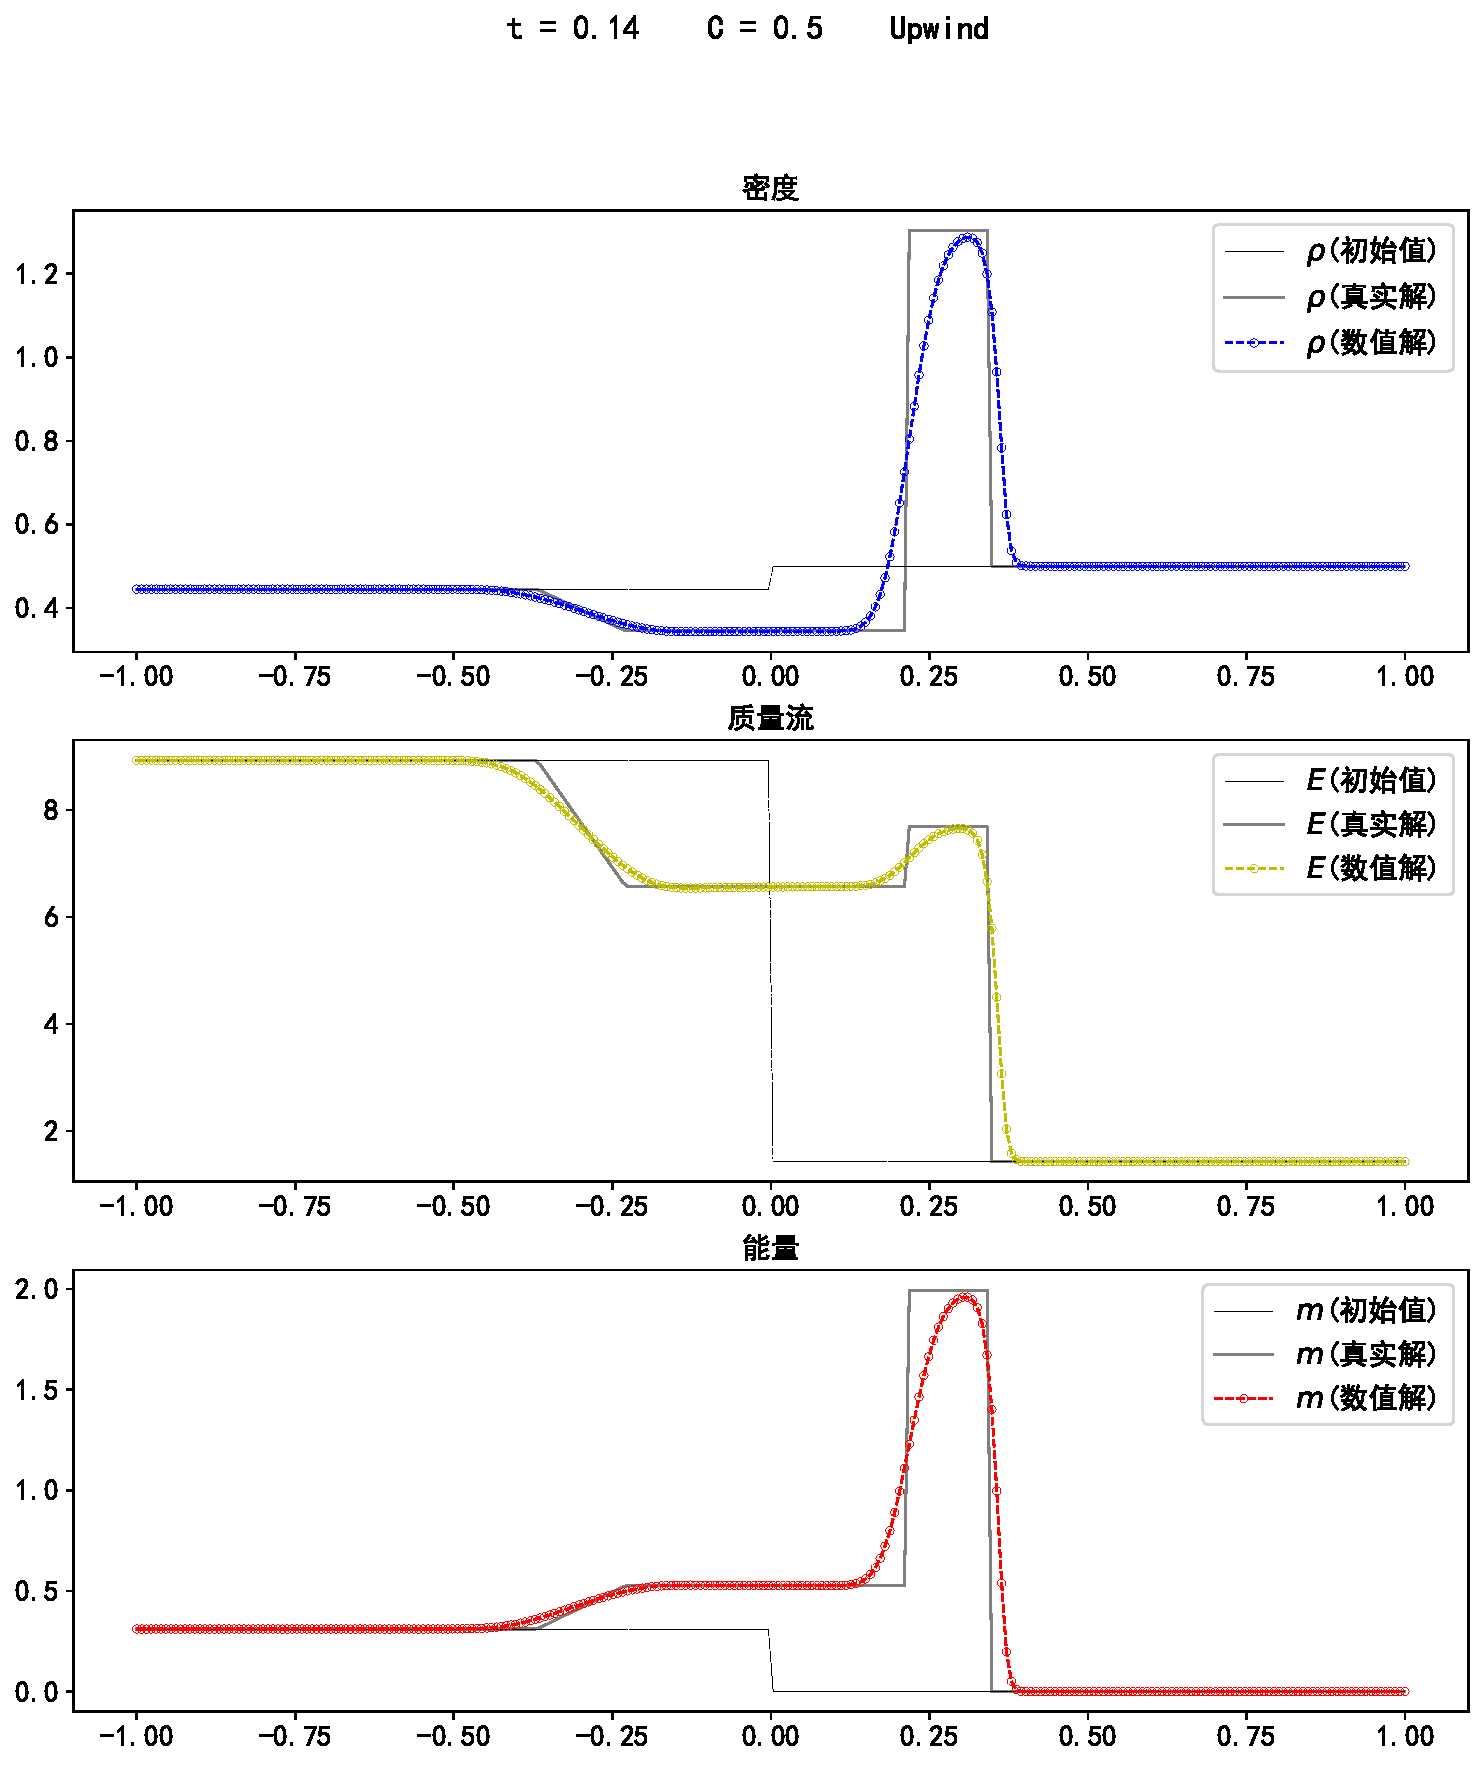
\includegraphics[width=.85\textwidth]{figures/upwind261.pdf}
\caption{迎风格式计算结果, 网格点数为 261. \textbf{从上到下分别是密度 $\rho$, 能量 $E$ 和质量流 $m = \rho u$.}
其中点线是初值, 虚线 (上面的数据点用符号 $\circ$ 标注) 是 $t=0.14$ 时的数值结果, 实线是对应的真实解.}\label{fig:Upwind}
\end{center}
\end{figure}

\subsection{\textit{TVD}格式}
\textit{TVD}格式适用于非守恒方程
\begin{align}
\pdv{\vb u}{t} + \vb*B \vdot \pdv{\vb u}{x} = 0
\end{align}
\textit{TVD}全称为\textit{Total Variat Diminishing},即总变差不变或减小,代表着震荡的剧烈程度减少,能保证迭代过程中不发散。其中\textit{Minmod}为某一种TVD格式,也是这次实验所采用的方法。
\textit{Minmod}差分形式为
\begin{equation}
\begin{aligned}
u_{k,l}^{n+1} &= u_{k,l}^n \\
& - \frac{\Delta t}{\Delta x} \sum_i \sum_j \bigg\{\text{sgn}(\lambda_{i,l}^n)
 \lambda_{i,l}^n R_{ki,l}^n L_{ij,l}^n \left[u_{j,l}^n - u_{j,l-\text{sgn}(\lambda_{i,l}^n)}^n\right]\\
& - \frac{1}{2}
\text{sgn}(\lambda_{i,l}^n) \lambda_{i,l}^n R_{ki,l}^n L_{ij,l}^n
	\qty[\Delta x-\text{sgn}(\lambda_{i,l}^n) \lambda_{i,l}^n R_{ki,l}^n L_{ij,l}^n \Delta t]
 \left[\sigma_{j,l}^n - \sigma_{j,l-\text{sgn}(\lambda_{i,l}^n)}^n\right]\bigg\},
\end{aligned}
\end{equation}
其中
\begin{equation}
	\sigma_i^n = \verb|Minmod| \left( \frac{u_i^n - u_{i-1}^{n}}{ \Delta x }, \frac{u_{i+1}^n - u_{i}^{n}}{ \Delta x } \right),
\end{equation}
\begin{equation}
	\verb|Minmod|(a, b) = 
	\begin{cases}
		a, \qif |a| < |b| \qand ab > 0\\
		b, \qif |a| > |b| \qand ab > 0\\
		0, \qif ab \leq 0.
	\end{cases}
\end{equation}
我们发现由于 \textit{TVD} 格式较 \textit{Upwind} 格式而言会出现振荡,
导致 \(\rho\) 或 \(p\) 出现负值,则在 \(a = \sqrt{\gamma \rho / p}\) 中根号下出现负值,
我们调整 CFL 为 0.05 后进行了模拟,根号下便不再出现负值。

\begin{figure}
\begin{center}
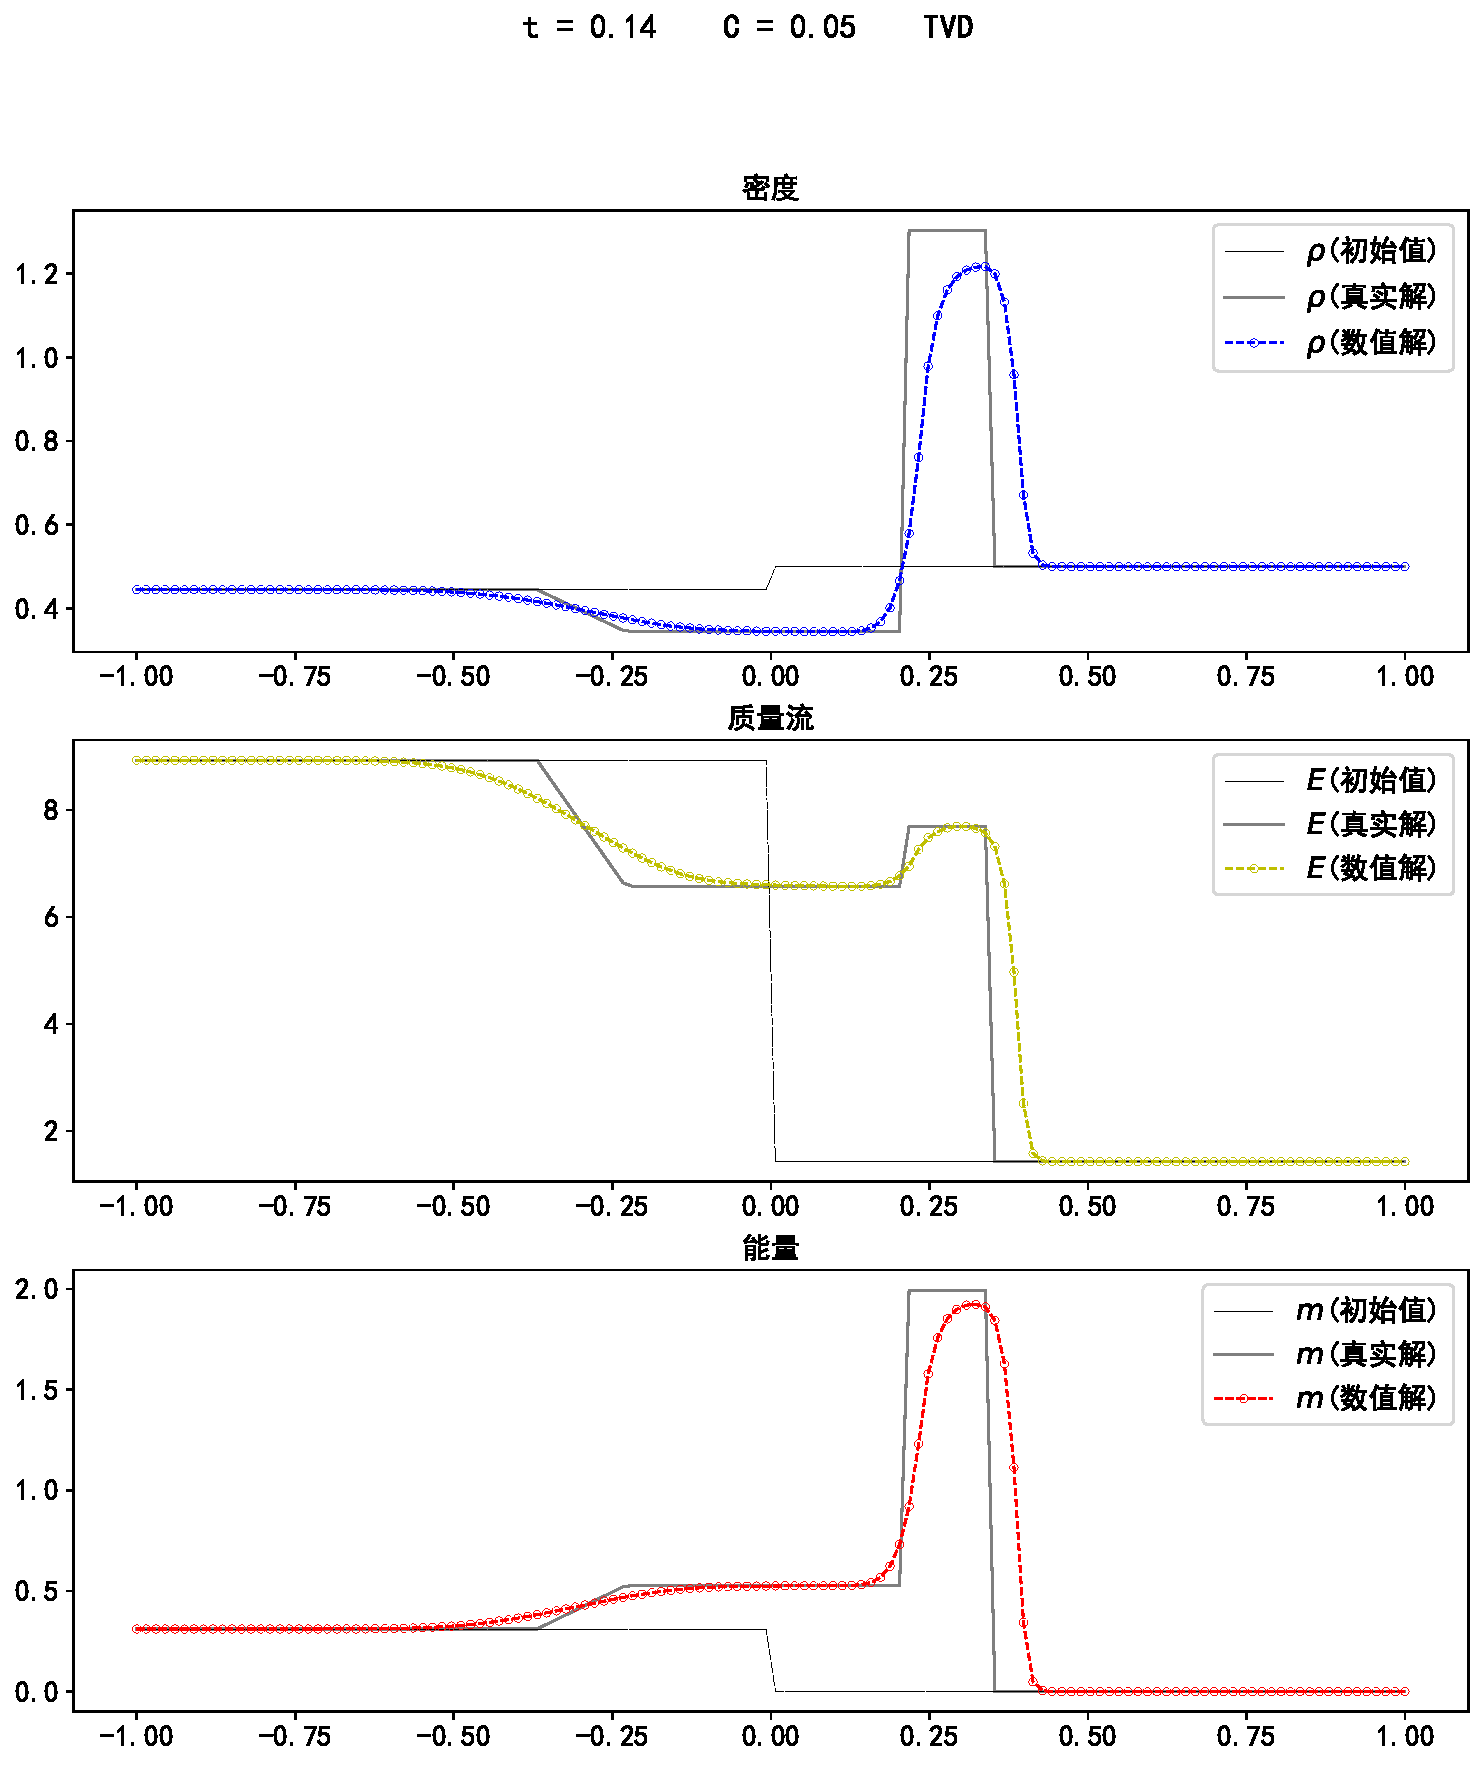
\includegraphics[width=.85\textwidth]{figures/limiter133.pdf}
\caption{(van Leer) TVD 格式计算结果, 网格点数为 133. 其他标注同图~\ref{fig:Upwind}.}\label{fig:vanLeerA}
\end{center}
\end{figure}

\begin{figure}
\begin{center}
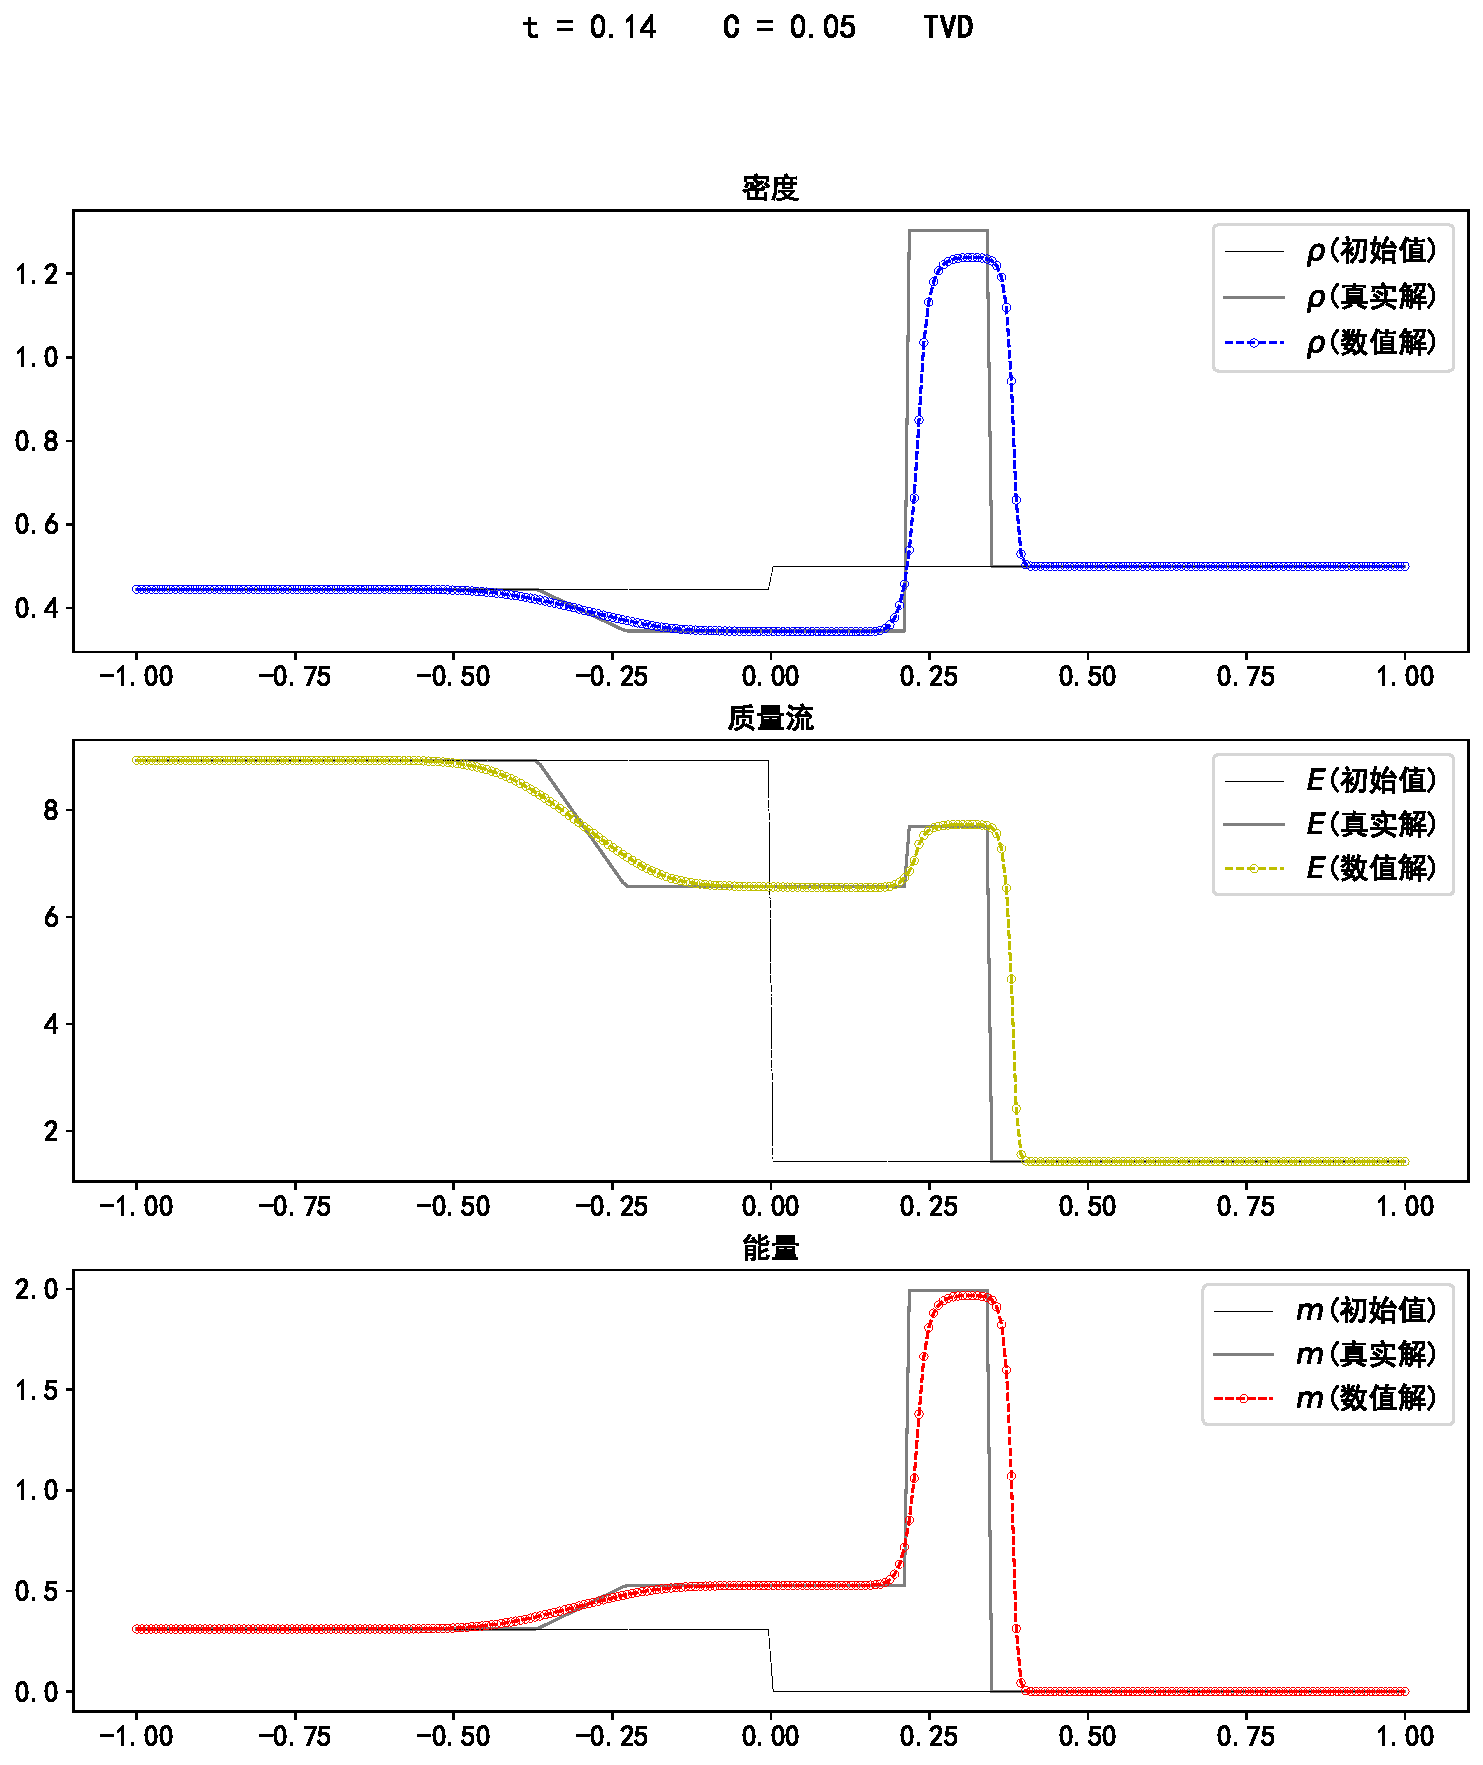
\includegraphics[width=.85\textwidth]{figures/limiter261.pdf}
\caption{(van Leer) TVD 格式计算结果, 网格点数为 261. 其他标注同图~\ref{fig:Upwind}.}\label{fig:vanLeerB}
\end{center}
\end{figure}
\subsection{实验结果分析与对比}

%设计两到三种有限差分格式, 编程进行数值计算, 给出图形, 比较和讨论结果. 或者, 利用附件中的 Excel 表格, 生成别的初值条件及解, 对流体力学中的间断问题进行数值计算并作进一步的讨论.

%作为参考, 这里给出三个算例, CFL 系数均取 0.5, $t=0.14$ 时刻的数值的计算结果. 迎风格式, 261 网格的数据如图~\ref{fig:Upwind},
%TVD (Total Variation Diminishing) 格式 \citep{vanLeer1974,Harten1983}, 133 网格的数据如图~\ref{fig:vanLeerA}, 以及 TVD 格式, 261
%网格的数据如图~\ref{fig:vanLeerB}. 供大家参考.


\begin{itemize}
	\item
Lax-Wendroff的实验格式如图~\ref{fig:lax_wendroff}~所示,
各物理量高度保持得很好,
过渡区间宽度与解析解基本一致,
但出现的色散 (上冲和下冲),在间断处出现振荡。

\item
\textit{Upwind}的实验格式结果如图~\ref{fig:Upwind}~所示,
物理量随着波的传播被逐渐抹平,过渡区间宽度较长。

\item
\textit{TVD}的实验格式结果如图~\ref{fig:vanLeerA}~和图~\ref{fig:vanLeerB}~所示,
由于 \textit{Minmod} 格式存在高阶补偿项,存在色散,能够较快速度将激波间隔缩小到2个左右的间隔距离,
就激波模拟而言 \textit{Minmod} 格式比 \textit{UpWind} 格式存在一定的优势。
\begin{itemize}
	\item 格点数为 133 的 TVD 格式(图~\ref{fig:vanLeerA})较格点数为 261 的 TVD 格式(图~\ref{fig:vanLeerB})间断点处更平滑无棱角。
\end{itemize}

\end{itemize}
\section{分工说明}
余航编写了代码main.py与run.sh,徐均益编写了main.jl,两人独立实现了守恒形式与非守恒形式的数值代码编写并共同调试,还包括\textit{Minmod}等满足TVD的限制器格式。
 余航、徐均益、陈宇韬进行了文档编写和校验。
\section{附件}

\begin{enumerate}
% \verb|code/Upwind格式svd验证.nb|
% \verb|figures/lax_wendroff261.pdf|
% \verb|figures/limiter0133.pdf|
% \verb|figures/limiter0261.pdf|
% \verb|figures/upwind00261.pdf|
% \verb|figures/upwind0261.pdf|
% \verb|figures/upwind_non0261.pdf|
% \verb|figures/upwind_non261.pdf|

\item
\verb|main.tex|
-- 本报告 \LaTeX  文件.
\item
\verb|main.pdf|
-- 本报告 PDF 输出文件.
\item
\verb|code/main.jl|
--  徐均益编写的 julia 代码
\item
\verb|code/main.py| 和 
\verb|code/run.sh|
--  分别是余航编写的 python 代码和 bash 运行脚本
\item
\verb|References.bib|
--  文献文件
\item
\verb|figures/upwind261.pdf|
-- 迎风格式计算结果, 261 网格.
\item
\verb|figures/limiter133.pdf|
-- van Leer TVD 格式计算结果, 133 网格.
\item
\verb|figures/limiter261.pdf|
-- van Leer TVD 格式计算结果, 261 网格.
\item
\verb|Hydrodynamics.xlsx|
-- 相关问题 Excel 计算表格, 深绿色单元为输入, 可以变更. 其中

\begin{enumerate}
\item
  Riemann 表格中, B2 为 $\gamma$ 值, B4-- B6 和 E4--E6 分别是左侧和右侧的密度, 质量流及能量的初值. A25--A26 迭代用值, A24 为 A25 和 A26 的平均值.
  22 行复制 24 行的值. 当 G24, 即 G22 值为零时, 得到此 Riemann 问题的解. N3 为时间值, 密度, 质量流及能量图形的坐标初值和对应比例分别由 N4-- N6 和 O4--O6 调节.
\item
Hydrodynamics 表格为对应守恒型方程的矩阵特征值, 左右特征向量, 变量在各个波模的分解, 等等. 这些可以用于检查后续高精度格式计算的一些中间结果是否正确.
\end{enumerate}
\end{enumerate}

\bibliographystyle{apalike}
\bibliography{References}

\end{document}
